\documentclass[1p]{elsarticle_modified}
%\bibliographystyle{elsarticle-num}

%\usepackage[colorlinks]{hyperref}
%\usepackage{abbrmath_seonhwa} %\Abb, \Ascr, \Acal ,\Abf, \Afrak
\usepackage{amsfonts}
\usepackage{amssymb}
\usepackage{amsmath}
\usepackage{amsthm}
\usepackage{scalefnt}
\usepackage{amsbsy}
\usepackage{kotex}
\usepackage{caption}
\usepackage{subfig}
\usepackage{color}
\usepackage{graphicx}
\usepackage{xcolor} %% white, black, red, green, blue, cyan, magenta, yellow
\usepackage{float}
\usepackage{setspace}
\usepackage{hyperref}

\usepackage{tikz}
\usetikzlibrary{arrows}

\usepackage{multirow}
\usepackage{array} % fixed length table
\usepackage{hhline}

%%%%%%%%%%%%%%%%%%%%%
\makeatletter
\renewcommand*\env@matrix[1][\arraystretch]{%
	\edef\arraystretch{#1}%
	\hskip -\arraycolsep
	\let\@ifnextchar\new@ifnextchar
	\array{*\c@MaxMatrixCols c}}
\makeatother %https://tex.stackexchange.com/questions/14071/how-can-i-increase-the-line-spacing-in-a-matrix
%%%%%%%%%%%%%%%

\usepackage[normalem]{ulem}

\newcommand{\msout}[1]{\ifmmode\text{\sout{\ensuremath{#1}}}\else\sout{#1}\fi}
%SOURCE: \msout is \stkout macro in https://tex.stackexchange.com/questions/20609/strikeout-in-math-mode

\newcommand{\cancel}[1]{
	\ifmmode
	{\color{red}\msout{#1}}
	\else
	{\color{red}\sout{#1}}
	\fi
}

\newcommand{\add}[1]{
	{\color{blue}\uwave{#1}}
}

\newcommand{\replace}[2]{
	\ifmmode
	{\color{red}\msout{#1}}{\color{blue}\uwave{#2}}
	\else
	{\color{red}\sout{#1}}{\color{blue}\uwave{#2}}
	\fi
}

\newcommand{\Sol}{\mathcal{S}} %segment
\newcommand{\D}{D} %diagram
\newcommand{\A}{\mathcal{A}} %arc


%%%%%%%%%%%%%%%%%%%%%%%%%%%%%5 test

\def\sl{\operatorname{\textup{SL}}(2,\Cbb)}
\def\psl{\operatorname{\textup{PSL}}(2,\Cbb)}
\def\quan{\mkern 1mu \triangleright \mkern 1mu}

\theoremstyle{definition}
\newtheorem{thm}{Theorem}[section]
\newtheorem{prop}[thm]{Proposition}
\newtheorem{lem}[thm]{Lemma}
\newtheorem{ques}[thm]{Question}
\newtheorem{cor}[thm]{Corollary}
\newtheorem{defn}[thm]{Definition}
\newtheorem{exam}[thm]{Example}
\newtheorem{rmk}[thm]{Remark}
\newtheorem{alg}[thm]{Algorithm}

\newcommand{\I}{\sqrt{-1}}
\begin{document}

%\begin{frontmatter}
%
%\title{Boundary parabolic representations of knots up to 8 crossings}
%
%%% Group authors per affiliation:
%\author{Yunhi Cho} 
%\address{Department of Mathematics, University of Seoul, Seoul, Korea}
%\ead{yhcho@uos.ac.kr}
%
%
%\author{Seonhwa Kim} %\fnref{s_kim}}
%\address{Center for Geometry and Physics, Institute for Basic Science, Pohang, 37673, Korea}
%\ead{ryeona17@ibs.re.kr}
%
%\author{Hyuk Kim}
%\address{Department of Mathematical Sciences, Seoul National University, Seoul 08826, Korea}
%\ead{hyukkim@snu.ac.kr}
%
%\author{Seokbeom Yoon}
%\address{Department of Mathematical Sciences, Seoul National University, Seoul, 08826,  Korea}
%\ead{sbyoon15@snu.ac.kr}
%
%\begin{abstract}
%We find all boundary parabolic representation of knots up to 8 crossings.
%
%\end{abstract}
%\begin{keyword}
%    \MSC[2010] 57M25 
%\end{keyword}
%
%\end{frontmatter}

%\linenumbers
%\tableofcontents
%
\newcommand\colored[1]{\textcolor{white}{\rule[-0.35ex]{0.8em}{1.4ex}}\kern-0.8em\color{red} #1}%
%\newcommand\colored[1]{\textcolor{white}{ #1}\kern-2.17ex	\textcolor{white}{ #1}\kern-1.81ex	\textcolor{white}{ #1}\kern-2.15ex\color{red}#1	}

{\Large $\underline{12n_{0743}~(K12n_{0743})}$}

\setlength{\tabcolsep}{10pt}
\renewcommand{\arraystretch}{1.6}
\vspace{1cm}\begin{tabular}{m{100pt}>{\centering\arraybackslash}m{274pt}}
\multirow{5}{120pt}{
	\centering
	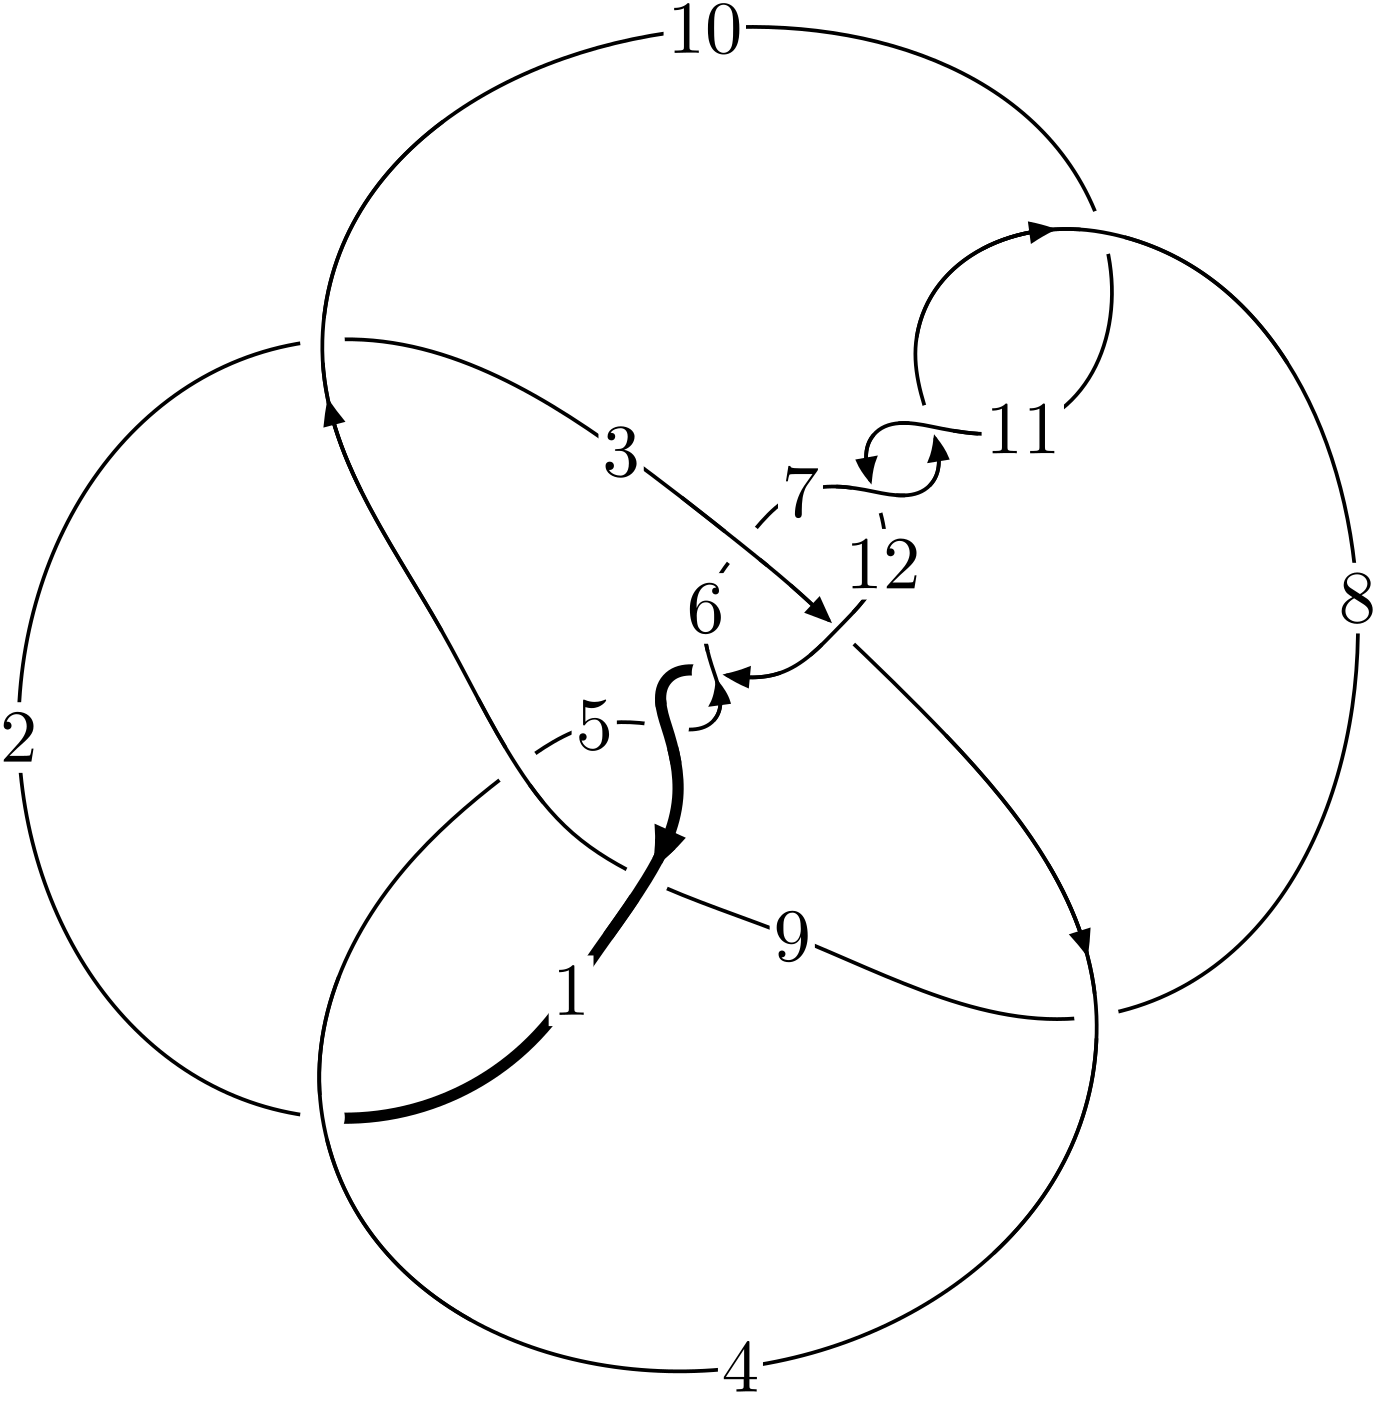
\includegraphics[width=112pt]{../../../GIT/diagram.site/Diagrams/png/2832_12n_0743.png}\\
\ \ \ A knot diagram\footnotemark}&
\allowdisplaybreaks
\textbf{Linearized knot diagam} \\
\cline{2-2}
 &
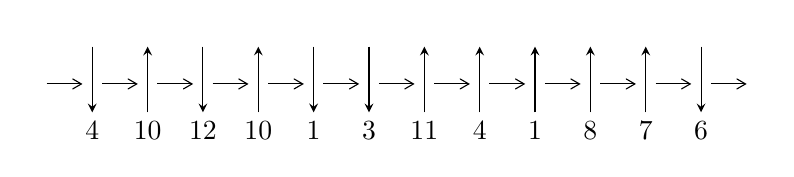
\begin{tikzpicture}[x=20pt, y=17pt]
	% nodes
	\node (C0) at (0, 0) {};
	\node (C1) at (1, 0) {};
	\node (C1U) at (1, +1) {};
	\node (C1D) at (1, -1) {4};

	\node (C2) at (2, 0) {};
	\node (C2U) at (2, +1) {};
	\node (C2D) at (2, -1) {10};

	\node (C3) at (3, 0) {};
	\node (C3U) at (3, +1) {};
	\node (C3D) at (3, -1) {12};

	\node (C4) at (4, 0) {};
	\node (C4U) at (4, +1) {};
	\node (C4D) at (4, -1) {10};

	\node (C5) at (5, 0) {};
	\node (C5U) at (5, +1) {};
	\node (C5D) at (5, -1) {1};

	\node (C6) at (6, 0) {};
	\node (C6U) at (6, +1) {};
	\node (C6D) at (6, -1) {3};

	\node (C7) at (7, 0) {};
	\node (C7U) at (7, +1) {};
	\node (C7D) at (7, -1) {11};

	\node (C8) at (8, 0) {};
	\node (C8U) at (8, +1) {};
	\node (C8D) at (8, -1) {4};

	\node (C9) at (9, 0) {};
	\node (C9U) at (9, +1) {};
	\node (C9D) at (9, -1) {1};

	\node (C10) at (10, 0) {};
	\node (C10U) at (10, +1) {};
	\node (C10D) at (10, -1) {8};

	\node (C11) at (11, 0) {};
	\node (C11U) at (11, +1) {};
	\node (C11D) at (11, -1) {7};

	\node (C12) at (12, 0) {};
	\node (C12U) at (12, +1) {};
	\node (C12D) at (12, -1) {6};
	\node (C13) at (13, 0) {};

	% arrows
	\draw[->,>={angle 60}]
	(C0) edge (C1) (C1) edge (C2) (C2) edge (C3) (C3) edge (C4) (C4) edge (C5) (C5) edge (C6) (C6) edge (C7) (C7) edge (C8) (C8) edge (C9) (C9) edge (C10) (C10) edge (C11) (C11) edge (C12) (C12) edge (C13) ;	\draw[->,>=stealth]
	(C1U) edge (C1D) (C2D) edge (C2U) (C3U) edge (C3D) (C4D) edge (C4U) (C5U) edge (C5D) (C6U) edge (C6D) (C7D) edge (C7U) (C8D) edge (C8U) (C9D) edge (C9U) (C10D) edge (C10U) (C11D) edge (C11U) (C12U) edge (C12D) ;
	\end{tikzpicture} \\
\hhline{~~} \\& 
\textbf{Solving Sequence} \\ \cline{2-2} 
 &
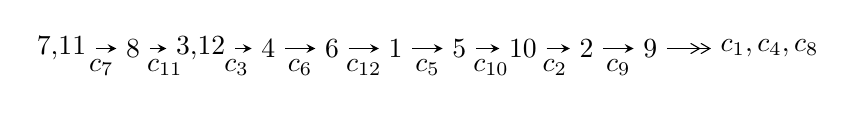
\begin{tikzpicture}[x=23pt, y=7pt]
	% node
	\node (A0) at (-1/8, 0) {7,11};
	\node (A1) at (1, 0) {8};
	\node (A2) at (33/16, 0) {3,12};
	\node (A3) at (25/8, 0) {4};
	\node (A4) at (33/8, 0) {6};
	\node (A5) at (41/8, 0) {1};
	\node (A6) at (49/8, 0) {5};
	\node (A7) at (57/8, 0) {10};
	\node (A8) at (65/8, 0) {2};
	\node (A9) at (73/8, 0) {9};
	\node (C1) at (1/2, -1) {$c_{7}$};
	\node (C2) at (3/2, -1) {$c_{11}$};
	\node (C3) at (21/8, -1) {$c_{3}$};
	\node (C4) at (29/8, -1) {$c_{6}$};
	\node (C5) at (37/8, -1) {$c_{12}$};
	\node (C6) at (45/8, -1) {$c_{5}$};
	\node (C7) at (53/8, -1) {$c_{10}$};
	\node (C8) at (61/8, -1) {$c_{2}$};
	\node (C9) at (69/8, -1) {$c_{9}$};
	\node (A10) at (11, 0) {$c_{1},c_{4},c_{8}$};

	% edge
	\draw[->,>=stealth]	
	(A0) edge (A1) (A1) edge (A2) (A2) edge (A3) (A3) edge (A4) (A4) edge (A5) (A5) edge (A6) (A6) edge (A7) (A7) edge (A8) (A8) edge (A9) ;
	\draw[->>,>={angle 60}]	
	(A9) edge (A10);
\end{tikzpicture} \\ 

\end{tabular} \\

\footnotetext{
The image of knot diagram is generated by the software ``\textbf{Draw programme}" developed by Andrew Bartholomew(\url{http://www.layer8.co.uk/maths/draw/index.htm\#Running-draw}), where we modified some parts for our purpose(\url{https://github.com/CATsTAILs/LinksPainter}).
}\phantom \\ \newline 
\centering \textbf{Ideals for irreducible components\footnotemark of $X_{\text{par}}$} 
 
\begin{align*}
I^u_{1}&=\langle 
-5 u^{24}+40 u^{23}+\cdots+2 b+42,\;11 u^{24}-78 u^{23}+\cdots+4 a+44,\;u^{25}-8 u^{24}+\cdots-42 u+4\rangle \\
I^u_{2}&=\langle 
-424456 u^7 a^3-1015802 u^7 a^2+\cdots-1966550 a-824409,\;5 u^7 a^2-3 u^7+\cdots+6 a+5,\\
\phantom{I^u_{2}}&\phantom{= \langle  }u^8+u^7+5 u^6+4 u^5+7 u^4+4 u^3+2 u^2+1\rangle \\
I^u_{3}&=\langle 
- u^{12}-2 u^{11}-8 u^{10}-13 u^9-24 u^8-30 u^7-31 u^6-26 u^5-12 u^4-3 u^3+4 u^2+b+2 u,\\
\phantom{I^u_{3}}&\phantom{= \langle  }- u^{12}-3 u^{11}-10 u^{10}-21 u^9-37 u^8-54 u^7-61 u^6-57 u^5-38 u^4-15 u^3+u^2+a+6 u+2,\\
\phantom{I^u_{3}}&\phantom{= \langle  }u^{15}+3 u^{14}+\cdots+u^2+1\rangle \\
\\
\end{align*}
\raggedright * 3 irreducible components of $\dim_{\mathbb{C}}=0$, with total 72 representations.\\
\footnotetext{All coefficients of polynomials are rational numbers. But the coefficients are sometimes approximated in decimal forms when there is not enough margin.}
\newpage
\renewcommand{\arraystretch}{1}
\centering \section*{I. $I^u_{1}= \langle -5 u^{24}+40 u^{23}+\cdots+2 b+42,\;11 u^{24}-78 u^{23}+\cdots+4 a+44,\;u^{25}-8 u^{24}+\cdots-42 u+4 \rangle$}
\flushleft \textbf{(i) Arc colorings}\\
\begin{tabular}{m{7pt} m{180pt} m{7pt} m{180pt} }
\flushright $a_{7}=$&$\begin{pmatrix}1\\0\end{pmatrix}$ \\
\flushright $a_{11}=$&$\begin{pmatrix}0\\u\end{pmatrix}$ \\
\flushright $a_{8}=$&$\begin{pmatrix}1\\- u^2\end{pmatrix}$ \\
\flushright $a_{3}=$&$\begin{pmatrix}-\frac{11}{4} u^{24}+\frac{39}{2} u^{23}+\cdots+\frac{153}{4} u-11\\\frac{5}{2} u^{24}-20 u^{23}+\cdots+\frac{421}{2} u-21\end{pmatrix}$ \\
\flushright $a_{12}=$&$\begin{pmatrix}u\\u\end{pmatrix}$ \\
\flushright $a_{4}=$&$\begin{pmatrix}-\frac{11}{4} u^{24}+\frac{39}{2} u^{23}+\cdots-\frac{183}{4} u-1\\\frac{5}{2} u^{24}-20 u^{23}+\cdots+\frac{253}{2} u-11\end{pmatrix}$ \\
\flushright $a_{6}=$&$\begin{pmatrix}\frac{3}{2} u^{24}-\frac{25}{2} u^{23}+\cdots+\frac{297}{2} u-\frac{31}{2}\\\frac{3}{2} u^{24}-11 u^{23}+\cdots-132 u^2+\frac{33}{2} u\end{pmatrix}$ \\
\flushright $a_{1}=$&$\begin{pmatrix}-\frac{15}{4} u^{24}+\frac{57}{2} u^{23}+\cdots-\frac{815}{4} u+19\\\frac{3}{2} u^{24}-13 u^{23}+\cdots+\frac{477}{2} u-27\end{pmatrix}$ \\
\flushright $a_{5}=$&$\begin{pmatrix}\frac{11}{4} u^{24}-\frac{39}{2} u^{23}+\cdots+\frac{247}{4} u-1\\-\frac{5}{2} u^{24}+20 u^{23}+\cdots-\frac{285}{2} u+13\end{pmatrix}$ \\
\flushright $a_{10}=$&$\begin{pmatrix}- u\\u^3+u\end{pmatrix}$ \\
\flushright $a_{2}=$&$\begin{pmatrix}-\frac{3}{4} u^{24}+\frac{9}{2} u^{23}+\cdots+\frac{401}{4} u-17\\\frac{5}{2} u^{24}-19 u^{23}+\cdots+\frac{229}{2} u-11\end{pmatrix}$ \\
\flushright $a_{9}=$&$\begin{pmatrix}\frac{3}{2} u^{24}-\frac{23}{2} u^{23}+\cdots+\frac{163}{2} u-\frac{15}{2}\\-\frac{1}{2} u^{24}+4 u^{23}+\cdots-\frac{113}{2} u+6\end{pmatrix}$\\&\end{tabular}
\flushleft \textbf{(ii) Obstruction class $= -1$}\\~\\
\flushleft \textbf{(iii) Cusp Shapes $= u^{24}-7 u^{23}+36 u^{22}-132 u^{21}+395 u^{20}-976 u^{19}+2048 u^{18}-3675 u^{17}+5648 u^{16}-7378 u^{15}+7999 u^{14}-6778 u^{13}+3633 u^{12}+552 u^{11}-4251 u^{10}+6027 u^9-5445 u^8+3234 u^7-776 u^6-810 u^5+1221 u^4-894 u^3+414 u^2-118 u+14$}\\~\\
\newpage\renewcommand{\arraystretch}{1}
\flushleft \textbf{(iv) u-Polynomials at the component}\newline \\
\begin{tabular}{m{50pt}|m{274pt}}
Crossings & \hspace{64pt}u-Polynomials at each crossing \\
\hline $$\begin{aligned}c_{1}\end{aligned}$$&$\begin{aligned}
&u^{25}-18 u^{24}+\cdots+200 u-192
\end{aligned}$\\
\hline $$\begin{aligned}c_{2},c_{8}\end{aligned}$$&$\begin{aligned}
&u^{25}+u^{24}+\cdots+49 u-85
\end{aligned}$\\
\hline $$\begin{aligned}c_{3},c_{6}\end{aligned}$$&$\begin{aligned}
&u^{25}-4 u^{23}+\cdots+7 u-1
\end{aligned}$\\
\hline $$\begin{aligned}c_{4},c_{9}\end{aligned}$$&$\begin{aligned}
&u^{25}+17 u^{23}+\cdots+u-1
\end{aligned}$\\
\hline $$\begin{aligned}c_{5},c_{12}\end{aligned}$$&$\begin{aligned}
&u^{25}+16 u^{24}+\cdots-2816 u-256
\end{aligned}$\\
\hline $$\begin{aligned}c_{7},c_{10},c_{11}\end{aligned}$$&$\begin{aligned}
&u^{25}+8 u^{24}+\cdots-42 u-4
\end{aligned}$\\
\hline
\end{tabular}\\~\\
\newpage\renewcommand{\arraystretch}{1}
\flushleft \textbf{(v) Riley Polynomials at the component}\newline \\
\begin{tabular}{m{50pt}|m{274pt}}
Crossings & \hspace{64pt}Riley Polynomials at each crossing \\
\hline $$\begin{aligned}c_{1}\end{aligned}$$&$\begin{aligned}
&y^{25}-28 y^{24}+\cdots+395968 y-36864
\end{aligned}$\\
\hline $$\begin{aligned}c_{2},c_{8}\end{aligned}$$&$\begin{aligned}
&y^{25}+23 y^{24}+\cdots-26159 y-7225
\end{aligned}$\\
\hline $$\begin{aligned}c_{3},c_{6}\end{aligned}$$&$\begin{aligned}
&y^{25}-8 y^{24}+\cdots+71 y-1
\end{aligned}$\\
\hline $$\begin{aligned}c_{4},c_{9}\end{aligned}$$&$\begin{aligned}
&y^{25}+34 y^{24}+\cdots-11 y-1
\end{aligned}$\\
\hline $$\begin{aligned}c_{5},c_{12}\end{aligned}$$&$\begin{aligned}
&y^{25}+14 y^{24}+\cdots+393216 y-65536
\end{aligned}$\\
\hline $$\begin{aligned}c_{7},c_{10},c_{11}\end{aligned}$$&$\begin{aligned}
&y^{25}+26 y^{24}+\cdots-164 y-16
\end{aligned}$\\
\hline
\end{tabular}\\~\\
\newpage\flushleft \textbf{(vi) Complex Volumes and Cusp Shapes}
$$\begin{array}{c|c|c}  
\text{Solutions to }I^u_{1}& \I (\text{vol} + \sqrt{-1}CS) & \text{Cusp shape}\\
 \hline 
\begin{aligned}
u &= \phantom{-}0.921555 + 0.389569 I \\
a &= -0.228724 + 0.336449 I \\
b &= \phantom{-}0.714884 + 0.733561 I\end{aligned}
 & -3.72259 - 5.55262 I & \phantom{-}1.00846 + 5.11814 I \\ \hline\begin{aligned}
u &= \phantom{-}0.921555 - 0.389569 I \\
a &= -0.228724 - 0.336449 I \\
b &= \phantom{-}0.714884 - 0.733561 I\end{aligned}
 & -3.72259 + 5.55262 I & \phantom{-}1.00846 - 5.11814 I \\ \hline\begin{aligned}
u &= \phantom{-}0.754292 + 0.675553 I \\
a &= \phantom{-}0.935089 + 0.407093 I \\
b &= \phantom{-}1.02266 - 1.00894 I\end{aligned}
 & -4.63523 + 10.99550 I & \phantom{-}0.61931 - 7.61444 I \\ \hline\begin{aligned}
u &= \phantom{-}0.754292 - 0.675553 I \\
a &= \phantom{-}0.935089 - 0.407093 I \\
b &= \phantom{-}1.02266 + 1.00894 I\end{aligned}
 & -4.63523 - 10.99550 I & \phantom{-}0.61931 + 7.61444 I \\ \hline\begin{aligned}
u &= \phantom{-}0.911256 + 0.682747 I \\
a &= -0.409833 - 0.368341 I \\
b &= -0.863640 + 0.290917 I\end{aligned}
 & -8.28803 + 3.15505 I & -4.81935 - 5.19613 I \\ \hline\begin{aligned}
u &= \phantom{-}0.911256 - 0.682747 I \\
a &= -0.409833 + 0.368341 I \\
b &= -0.863640 - 0.290917 I\end{aligned}
 & -8.28803 - 3.15505 I & -4.81935 + 5.19613 I \\ \hline\begin{aligned}
u &= -0.781714\phantom{ +0.000000I} \\
a &= -0.294872\phantom{ +0.000000I} \\
b &= -0.129373\phantom{ +0.000000I}\end{aligned}
 & \phantom{-}1.14840\phantom{ +0.000000I} & \phantom{-}15.4840\phantom{ +0.000000I} \\ \hline\begin{aligned}
u &= \phantom{-}0.160604 + 0.683864 I \\
a &= \phantom{-}0.447358 - 1.171790 I \\
b &= -0.556568 - 0.593706 I\end{aligned}
 & \phantom{-}2.37371 - 1.53413 I & \phantom{-}1.38623 + 4.98201 I \\ \hline\begin{aligned}
u &= \phantom{-}0.160604 - 0.683864 I \\
a &= \phantom{-}0.447358 + 1.171790 I \\
b &= -0.556568 + 0.593706 I\end{aligned}
 & \phantom{-}2.37371 + 1.53413 I & \phantom{-}1.38623 - 4.98201 I \\ \hline\begin{aligned}
u &= -0.03035 + 1.46200 I \\
a &= -0.958194 - 0.059340 I \\
b &= -0.676699 + 0.397676 I\end{aligned}
 & -4.72338 - 2.11817 I & \phantom{-}0.56869 + 3.89890 I\\
 \hline 
 \end{array}$$\newpage$$\begin{array}{c|c|c}  
\text{Solutions to }I^u_{1}& \I (\text{vol} + \sqrt{-1}CS) & \text{Cusp shape}\\
 \hline 
\begin{aligned}
u &= -0.03035 - 1.46200 I \\
a &= -0.958194 + 0.059340 I \\
b &= -0.676699 - 0.397676 I\end{aligned}
 & -4.72338 + 2.11817 I & \phantom{-}0.56869 - 3.89890 I \\ \hline\begin{aligned}
u &= \phantom{-}0.05488 + 1.48295 I \\
a &= \phantom{-}1.56598 + 0.02201 I \\
b &= \phantom{-}1.097930 - 0.735677 I\end{aligned}
 & -7.25788 + 1.53536 I & -4.26963 - 0.95697 I \\ \hline\begin{aligned}
u &= \phantom{-}0.05488 - 1.48295 I \\
a &= \phantom{-}1.56598 - 0.02201 I \\
b &= \phantom{-}1.097930 + 0.735677 I\end{aligned}
 & -7.25788 - 1.53536 I & -4.26963 + 0.95697 I \\ \hline\begin{aligned}
u &= \phantom{-}0.09014 + 1.48837 I \\
a &= -1.94282 + 0.27279 I \\
b &= -1.22851 + 1.14146 I\end{aligned}
 & -2.73659 + 5.21328 I & -0.241059 - 0.933200 I \\ \hline\begin{aligned}
u &= \phantom{-}0.09014 - 1.48837 I \\
a &= -1.94282 - 0.27279 I \\
b &= -1.22851 - 1.14146 I\end{aligned}
 & -2.73659 - 5.21328 I & -0.241059 + 0.933200 I \\ \hline\begin{aligned}
u &= \phantom{-}0.365223 + 0.343863 I \\
a &= -0.89848 - 1.63604 I \\
b &= -0.883594 + 0.949370 I\end{aligned}
 & \phantom{-}3.39737 + 3.68728 I & -2.66049 - 0.54617 I \\ \hline\begin{aligned}
u &= \phantom{-}0.365223 - 0.343863 I \\
a &= -0.89848 + 1.63604 I \\
b &= -0.883594 - 0.949370 I\end{aligned}
 & \phantom{-}3.39737 - 3.68728 I & -2.66049 + 0.54617 I \\ \hline\begin{aligned}
u &= \phantom{-}0.24700 + 1.59114 I \\
a &= \phantom{-}1.88690 - 0.20760 I \\
b &= \phantom{-}1.32178 - 1.12604 I\end{aligned}
 & -12.1188 + 14.7263 I & -1.91172 - 6.80862 I \\ \hline\begin{aligned}
u &= \phantom{-}0.24700 - 1.59114 I \\
a &= \phantom{-}1.88690 + 0.20760 I \\
b &= \phantom{-}1.32178 + 1.12604 I\end{aligned}
 & -12.1188 - 14.7263 I & -1.91172 + 6.80862 I \\ \hline\begin{aligned}
u &= \phantom{-}0.203322 + 0.330620 I \\
a &= \phantom{-}0.46453 + 1.62148 I \\
b &= \phantom{-}0.687664 - 0.321221 I\end{aligned}
 & -1.185540 + 0.658151 I & -5.01541 - 1.91955 I\\
 \hline 
 \end{array}$$\newpage$$\begin{array}{c|c|c}  
\text{Solutions to }I^u_{1}& \I (\text{vol} + \sqrt{-1}CS) & \text{Cusp shape}\\
 \hline 
\begin{aligned}
u &= \phantom{-}0.203322 - 0.330620 I \\
a &= \phantom{-}0.46453 - 1.62148 I \\
b &= \phantom{-}0.687664 + 0.321221 I\end{aligned}
 & -1.185540 - 0.658151 I & -5.01541 + 1.91955 I \\ \hline\begin{aligned}
u &= \phantom{-}0.27991 + 1.60858 I \\
a &= -1.43237 - 0.19401 I \\
b &= -1.200770 + 0.592773 I\end{aligned}
 & -15.8446 + 7.4948 I & -4.78217 - 4.06320 I \\ \hline\begin{aligned}
u &= \phantom{-}0.27991 - 1.60858 I \\
a &= -1.43237 + 0.19401 I \\
b &= -1.200770 - 0.592773 I\end{aligned}
 & -15.8446 - 7.4948 I & -4.78217 + 4.06320 I \\ \hline\begin{aligned}
u &= \phantom{-}0.43302 + 1.62881 I \\
a &= \phantom{-}0.467991 + 0.457927 I \\
b &= \phantom{-}0.629543 + 0.114371 I\end{aligned}
 & -9.98504 - 0.27176 I & -10.12478 + 1.72289 I \\ \hline\begin{aligned}
u &= \phantom{-}0.43302 - 1.62881 I \\
a &= \phantom{-}0.467991 - 0.457927 I \\
b &= \phantom{-}0.629543 - 0.114371 I\end{aligned}
 & -9.98504 + 0.27176 I & -10.12478 - 1.72289 I\\
 \hline 
 \end{array}$$\newpage\newpage\renewcommand{\arraystretch}{1}
\centering \section*{II. $I^u_{2}= \langle -4.24\times10^{5} a^{3} u^{7}-1.02\times10^{6} a^{2} u^{7}+\cdots-1.97\times10^{6} a-8.24\times10^{5},\;5 u^7 a^2-3 u^7+\cdots+6 a+5,\;u^8+u^7+5 u^6+4 u^5+7 u^4+4 u^3+2 u^2+1 \rangle$}
\flushleft \textbf{(i) Arc colorings}\\
\begin{tabular}{m{7pt} m{180pt} m{7pt} m{180pt} }
\flushright $a_{7}=$&$\begin{pmatrix}1\\0\end{pmatrix}$ \\
\flushright $a_{11}=$&$\begin{pmatrix}0\\u\end{pmatrix}$ \\
\flushright $a_{8}=$&$\begin{pmatrix}1\\- u^2\end{pmatrix}$ \\
\flushright $a_{3}=$&$\begin{pmatrix}a\\0.214472 a^{3} u^{7}+0.513271 a^{2} u^{7}+\cdots+0.993671 a+0.416563\end{pmatrix}$ \\
\flushright $a_{12}=$&$\begin{pmatrix}u\\u\end{pmatrix}$ \\
\flushright $a_{4}=$&$\begin{pmatrix}-0.165445 a^{3} u^{7}-0.0257408 a^{2} u^{7}+\cdots+1.01296 a-0.199907\\0.0490264 a^{3} u^{7}+0.487530 a^{2} u^{7}+\cdots+1.00663 a+0.216656\end{pmatrix}$ \\
\flushright $a_{6}=$&$\begin{pmatrix}-0.145990 a^{3} u^{7}-0.157999 a^{2} u^{7}+\cdots+0.226482 a-0.0429312\\0.320279 a^{3} u^{7}+0.344935 a^{2} u^{7}+\cdots-1.00696 a-0.581214\end{pmatrix}$ \\
\flushright $a_{1}=$&$\begin{pmatrix}-0.223080 a^{3} u^{7}-0.106256 a^{2} u^{7}+\cdots-0.939315 a+0.0492462\\0.243189 a^{3} u^{7}+0.396678 a^{2} u^{7}+\cdots-2.17276 a-0.489037\end{pmatrix}$ \\
\flushright $a_{5}=$&$\begin{pmatrix}-0.285211 a^{3} u^{7}-0.317493 a^{2} u^{7}+\cdots-0.363491 a-0.0576562\\0.181058 a^{3} u^{7}+0.185441 a^{2} u^{7}+\cdots-1.59693 a-0.595939\end{pmatrix}$ \\
\flushright $a_{10}=$&$\begin{pmatrix}- u\\u^3+u\end{pmatrix}$ \\
\flushright $a_{2}=$&$\begin{pmatrix}-0.165445 a^{3} u^{7}-0.0257408 a^{2} u^{7}+\cdots+1.01296 a-0.199907\\0.164961 a^{3} u^{7}+0.644661 a^{2} u^{7}+\cdots+0.984109 a+0.398794\end{pmatrix}$ \\
\flushright $a_{9}=$&$\begin{pmatrix}-0.310215 a^{3} u^{7}-0.191868 a^{2} u^{7}+\cdots-0.160858 a-0.210923\\0.371570 a^{3} u^{7}+0.332317 a^{2} u^{7}+\cdots-1.85032 a-0.481154\end{pmatrix}$\\&\end{tabular}
\flushleft \textbf{(ii) Obstruction class $= -1$}\\~\\
\flushleft \textbf{(iii) Cusp Shapes $= -\frac{51112}{282725} u^7 a^3-\frac{399104}{282725} u^7 a^2+\cdots-\frac{27488}{11309} a-\frac{1177318}{282725}$}\\~\\
\newpage\renewcommand{\arraystretch}{1}
\flushleft \textbf{(iv) u-Polynomials at the component}\newline \\
\begin{tabular}{m{50pt}|m{274pt}}
Crossings & \hspace{64pt}u-Polynomials at each crossing \\
\hline $$\begin{aligned}c_{1}\end{aligned}$$&$\begin{aligned}
&(u^8+7 u^7+17 u^6+14 u^5- u^4+2 u^3+6 u^2-4 u+1)^4
\end{aligned}$\\
\hline $$\begin{aligned}c_{2},c_{8}\end{aligned}$$&$\begin{aligned}
&u^{32}- u^{31}+\cdots-18342 u+11689
\end{aligned}$\\
\hline $$\begin{aligned}c_{3},c_{6}\end{aligned}$$&$\begin{aligned}
&u^{32}+7 u^{31}+\cdots-32 u+7
\end{aligned}$\\
\hline $$\begin{aligned}c_{4},c_{9}\end{aligned}$$&$\begin{aligned}
&u^{32}- u^{31}+\cdots+2638 u+469
\end{aligned}$\\
\hline $$\begin{aligned}c_{5},c_{12}\end{aligned}$$&$\begin{aligned}
&(u^2- u+1)^{16}
\end{aligned}$\\
\hline $$\begin{aligned}c_{7},c_{10},c_{11}\end{aligned}$$&$\begin{aligned}
&(u^8- u^7+5 u^6-4 u^5+7 u^4-4 u^3+2 u^2+1)^4
\end{aligned}$\\
\hline
\end{tabular}\\~\\
\newpage\renewcommand{\arraystretch}{1}
\flushleft \textbf{(v) Riley Polynomials at the component}\newline \\
\begin{tabular}{m{50pt}|m{274pt}}
Crossings & \hspace{64pt}Riley Polynomials at each crossing \\
\hline $$\begin{aligned}c_{1}\end{aligned}$$&$\begin{aligned}
&(y^8-15 y^7+91 y^6-246 y^5+207 y^4+130 y^3+50 y^2-4 y+1)^4
\end{aligned}$\\
\hline $$\begin{aligned}c_{2},c_{8}\end{aligned}$$&$\begin{aligned}
&y^{32}+27 y^{31}+\cdots+2039149884 y+136632721
\end{aligned}$\\
\hline $$\begin{aligned}c_{3},c_{6}\end{aligned}$$&$\begin{aligned}
&y^{32}+3 y^{31}+\cdots-548 y+49
\end{aligned}$\\
\hline $$\begin{aligned}c_{4},c_{9}\end{aligned}$$&$\begin{aligned}
&y^{32}+35 y^{31}+\cdots-3846760 y+219961
\end{aligned}$\\
\hline $$\begin{aligned}c_{5},c_{12}\end{aligned}$$&$\begin{aligned}
&(y^2+y+1)^{16}
\end{aligned}$\\
\hline $$\begin{aligned}c_{7},c_{10},c_{11}\end{aligned}$$&$\begin{aligned}
&(y^8+9 y^7+31 y^6+50 y^5+39 y^4+22 y^3+18 y^2+4 y+1)^4
\end{aligned}$\\
\hline
\end{tabular}\\~\\
\newpage\flushleft \textbf{(vi) Complex Volumes and Cusp Shapes}
$$\begin{array}{c|c|c}  
\text{Solutions to }I^u_{2}& \I (\text{vol} + \sqrt{-1}CS) & \text{Cusp shape}\\
 \hline 
\begin{aligned}
u &= -0.647085 + 0.502738 I \\
a &= -0.608766 - 0.550255 I \\
b &= \phantom{-}0.182892 - 0.575506 I\end{aligned}
 & \phantom{-}1.67479 - 0.15547 I & \phantom{-}1.58319 - 0.32355 I \\ \hline\begin{aligned}
u &= -0.647085 + 0.502738 I \\
a &= -0.804300 + 0.904540 I \\
b &= -0.766883 - 0.706358 I\end{aligned}
 & \phantom{-}1.67479 - 4.21524 I & \phantom{-}1.58319 + 6.60465 I \\ \hline\begin{aligned}
u &= -0.647085 + 0.502738 I \\
a &= \phantom{-}0.575472 - 0.193692 I \\
b &= \phantom{-}0.785648 + 1.061200 I\end{aligned}
 & \phantom{-}1.67479 - 4.21524 I & \phantom{-}1.58319 + 6.60465 I \\ \hline\begin{aligned}
u &= -0.647085 + 0.502738 I \\
a &= \phantom{-}0.1075680 - 0.0033399 I \\
b &= -0.499575 + 0.414336 I\end{aligned}
 & \phantom{-}1.67479 - 0.15547 I & \phantom{-}1.58319 - 0.32355 I \\ \hline\begin{aligned}
u &= -0.647085 - 0.502738 I \\
a &= -0.608766 + 0.550255 I \\
b &= \phantom{-}0.182892 + 0.575506 I\end{aligned}
 & \phantom{-}1.67479 + 0.15547 I & \phantom{-}1.58319 + 0.32355 I \\ \hline\begin{aligned}
u &= -0.647085 - 0.502738 I \\
a &= -0.804300 - 0.904540 I \\
b &= -0.766883 + 0.706358 I\end{aligned}
 & \phantom{-}1.67479 + 4.21524 I & \phantom{-}1.58319 - 6.60465 I \\ \hline\begin{aligned}
u &= -0.647085 - 0.502738 I \\
a &= \phantom{-}0.575472 + 0.193692 I \\
b &= \phantom{-}0.785648 - 1.061200 I\end{aligned}
 & \phantom{-}1.67479 + 4.21524 I & \phantom{-}1.58319 - 6.60465 I \\ \hline\begin{aligned}
u &= -0.647085 - 0.502738 I \\
a &= \phantom{-}0.1075680 + 0.0033399 I \\
b &= -0.499575 - 0.414336 I\end{aligned}
 & \phantom{-}1.67479 + 0.15547 I & \phantom{-}1.58319 + 0.32355 I \\ \hline\begin{aligned}
u &= \phantom{-}0.283060 + 0.443755 I \\
a &= -0.741752 + 0.575430 I \\
b &= -0.28282 - 1.40078 I\end{aligned}
 & -4.93480 - 0.98388 I & -2.00000 - 3.22135 I \\ \hline\begin{aligned}
u &= \phantom{-}0.283060 + 0.443755 I \\
a &= \phantom{-}0.843131 + 0.210182 I \\
b &= \phantom{-}1.37494 + 1.03565 I\end{aligned}
 & -4.93480 + 3.07589 I & -2.00000 - 10.14955 I\\
 \hline 
 \end{array}$$\newpage$$\begin{array}{c|c|c}  
\text{Solutions to }I^u_{2}& \I (\text{vol} + \sqrt{-1}CS) & \text{Cusp shape}\\
 \hline 
\begin{aligned}
u &= \phantom{-}0.283060 + 0.443755 I \\
a &= \phantom{-}3.53954 + 0.62247 I \\
b &= \phantom{-}1.006860 - 0.355732 I\end{aligned}
 & -4.93480 - 0.98388 I & -2.00000 - 3.22135 I \\ \hline\begin{aligned}
u &= \phantom{-}0.283060 + 0.443755 I \\
a &= -3.27944 + 1.61382 I \\
b &= -0.215771 + 0.469647 I\end{aligned}
 & -4.93480 + 3.07589 I & -2.00000 - 10.14955 I \\ \hline\begin{aligned}
u &= \phantom{-}0.283060 - 0.443755 I \\
a &= -0.741752 - 0.575430 I \\
b &= -0.28282 + 1.40078 I\end{aligned}
 & -4.93480 + 0.98388 I & -2.00000 + 3.22135 I \\ \hline\begin{aligned}
u &= \phantom{-}0.283060 - 0.443755 I \\
a &= \phantom{-}0.843131 - 0.210182 I \\
b &= \phantom{-}1.37494 - 1.03565 I\end{aligned}
 & -4.93480 - 3.07589 I & -2.00000 + 10.14955 I \\ \hline\begin{aligned}
u &= \phantom{-}0.283060 - 0.443755 I \\
a &= \phantom{-}3.53954 - 0.62247 I \\
b &= \phantom{-}1.006860 + 0.355732 I\end{aligned}
 & -4.93480 + 0.98388 I & -2.00000 + 3.22135 I \\ \hline\begin{aligned}
u &= \phantom{-}0.283060 - 0.443755 I \\
a &= -3.27944 - 1.61382 I \\
b &= -0.215771 - 0.469647 I\end{aligned}
 & -4.93480 - 3.07589 I & -2.00000 + 10.14955 I \\ \hline\begin{aligned}
u &= \phantom{-}0.06382 + 1.51723 I \\
a &= -0.59184 - 1.50907 I \\
b &= -0.55330 - 2.21455 I\end{aligned}
 & -11.54440 + 0.15547 I & -5.58319 + 0.32355 I \\ \hline\begin{aligned}
u &= \phantom{-}0.06382 + 1.51723 I \\
a &= -1.44604 + 1.19889 I \\
b &= -0.332579 - 0.058640 I\end{aligned}
 & -11.54440 + 4.21524 I & -5.58319 - 6.60465 I \\ \hline\begin{aligned}
u &= \phantom{-}0.06382 + 1.51723 I \\
a &= \phantom{-}2.02681 + 1.39192 I \\
b &= \phantom{-}1.97903 + 1.60911 I\end{aligned}
 & -11.54440 + 4.21524 I & -5.58319 - 6.60465 I \\ \hline\begin{aligned}
u &= \phantom{-}0.06382 + 1.51723 I \\
a &= \phantom{-}2.54516 - 0.28930 I \\
b &= \phantom{-}1.072830 + 0.013443 I\end{aligned}
 & -11.54440 + 0.15547 I & -5.58319 + 0.32355 I\\
 \hline 
 \end{array}$$\newpage$$\begin{array}{c|c|c}  
\text{Solutions to }I^u_{2}& \I (\text{vol} + \sqrt{-1}CS) & \text{Cusp shape}\\
 \hline 
\begin{aligned}
u &= \phantom{-}0.06382 - 1.51723 I \\
a &= -0.59184 + 1.50907 I \\
b &= -0.55330 + 2.21455 I\end{aligned}
 & -11.54440 - 0.15547 I & -5.58319 - 0.32355 I \\ \hline\begin{aligned}
u &= \phantom{-}0.06382 - 1.51723 I \\
a &= -1.44604 - 1.19889 I \\
b &= -0.332579 + 0.058640 I\end{aligned}
 & -11.54440 - 4.21524 I & -5.58319 + 6.60465 I \\ \hline\begin{aligned}
u &= \phantom{-}0.06382 - 1.51723 I \\
a &= \phantom{-}2.02681 - 1.39192 I \\
b &= \phantom{-}1.97903 - 1.60911 I\end{aligned}
 & -11.54440 - 4.21524 I & -5.58319 + 6.60465 I \\ \hline\begin{aligned}
u &= \phantom{-}0.06382 - 1.51723 I \\
a &= \phantom{-}2.54516 + 0.28930 I \\
b &= \phantom{-}1.072830 - 0.013443 I\end{aligned}
 & -11.54440 - 0.15547 I & -5.58319 - 0.32355 I \\ \hline\begin{aligned}
u &= -0.19980 + 1.51366 I \\
a &= -1.337750 - 0.048574 I \\
b &= -1.080980 - 0.367558 I\end{aligned}
 & -4.93480 - 3.20880 I & -2.00000 - 0.42152 I \\ \hline\begin{aligned}
u &= -0.19980 + 1.51366 I \\
a &= \phantom{-}0.577550 - 0.281035 I \\
b &= \phantom{-}0.431533 + 0.452389 I\end{aligned}
 & -4.93480 - 3.20880 I & -2.00000 - 0.42152 I \\ \hline\begin{aligned}
u &= -0.19980 + 1.51366 I \\
a &= -1.71375 + 0.21126 I \\
b &= -0.977836 - 0.794944 I\end{aligned}
 & -4.93480 - 7.26857 I & -2.00000 + 6.50668 I \\ \hline\begin{aligned}
u &= -0.19980 + 1.51366 I \\
a &= \phantom{-}1.80840 + 0.61189 I \\
b &= \phantom{-}1.37603 + 1.31497 I\end{aligned}
 & -4.93480 - 7.26857 I & -2.00000 + 6.50668 I \\ \hline\begin{aligned}
u &= -0.19980 - 1.51366 I \\
a &= -1.337750 + 0.048574 I \\
b &= -1.080980 + 0.367558 I\end{aligned}
 & -4.93480 + 3.20880 I & -2.00000 + 0.42152 I \\ \hline\begin{aligned}
u &= -0.19980 - 1.51366 I \\
a &= \phantom{-}0.577550 + 0.281035 I \\
b &= \phantom{-}0.431533 - 0.452389 I\end{aligned}
 & -4.93480 + 3.20880 I & -2.00000 + 0.42152 I\\
 \hline 
 \end{array}$$\newpage$$\begin{array}{c|c|c}  
\text{Solutions to }I^u_{2}& \I (\text{vol} + \sqrt{-1}CS) & \text{Cusp shape}\\
 \hline 
\begin{aligned}
u &= -0.19980 - 1.51366 I \\
a &= -1.71375 - 0.21126 I \\
b &= -0.977836 + 0.794944 I\end{aligned}
 & -4.93480 + 7.26857 I & -2.00000 - 6.50668 I \\ \hline\begin{aligned}
u &= -0.19980 - 1.51366 I \\
a &= \phantom{-}1.80840 - 0.61189 I \\
b &= \phantom{-}1.37603 - 1.31497 I\end{aligned}
 & -4.93480 + 7.26857 I & -2.00000 - 6.50668 I\\
 \hline 
 \end{array}$$\newpage\newpage\renewcommand{\arraystretch}{1}
\centering \section*{III. $I^u_{3}= \langle - u^{12}-2 u^{11}+\cdots+b+2 u,\;- u^{12}-3 u^{11}+\cdots+a+2,\;u^{15}+3 u^{14}+\cdots+u^2+1 \rangle$}
\flushleft \textbf{(i) Arc colorings}\\
\begin{tabular}{m{7pt} m{180pt} m{7pt} m{180pt} }
\flushright $a_{7}=$&$\begin{pmatrix}1\\0\end{pmatrix}$ \\
\flushright $a_{11}=$&$\begin{pmatrix}0\\u\end{pmatrix}$ \\
\flushright $a_{8}=$&$\begin{pmatrix}1\\- u^2\end{pmatrix}$ \\
\flushright $a_{3}=$&$\begin{pmatrix}u^{12}+3 u^{11}+\cdots-6 u-2\\u^{12}+2 u^{11}+\cdots-4 u^2-2 u\end{pmatrix}$ \\
\flushright $a_{12}=$&$\begin{pmatrix}u\\u\end{pmatrix}$ \\
\flushright $a_{4}=$&$\begin{pmatrix}u^{13}+3 u^{12}+\cdots-6 u-2\\u^{13}+3 u^{12}+\cdots-6 u^2-2 u\end{pmatrix}$ \\
\flushright $a_{6}=$&$\begin{pmatrix}- u^{12}-3 u^{11}+\cdots-6 u-1\\- u^{12}-2 u^{11}+\cdots-4 u^2-2 u\end{pmatrix}$ \\
\flushright $a_{1}=$&$\begin{pmatrix}- u^{14}-4 u^{13}+\cdots+6 u+1\\- u^{13}-2 u^{12}+\cdots+u+1\end{pmatrix}$ \\
\flushright $a_{5}=$&$\begin{pmatrix}u^{13}+3 u^{12}+\cdots-6 u-2\\u^{13}+3 u^{12}+\cdots-3 u^2-2 u\end{pmatrix}$ \\
\flushright $a_{10}=$&$\begin{pmatrix}- u\\u^3+u\end{pmatrix}$ \\
\flushright $a_{2}=$&$\begin{pmatrix}u^{14}+3 u^{13}+\cdots-5 u-2\\u^{14}+3 u^{13}+\cdots-6 u^2-2 u\end{pmatrix}$ \\
\flushright $a_{9}=$&$\begin{pmatrix}- u^{14}-3 u^{13}+\cdots-37 u^2-9 u\\- u^9-3 u^8-8 u^7-15 u^6-21 u^5-24 u^4-19 u^3-10 u^2- u+1\end{pmatrix}$\\&\end{tabular}
\flushleft \textbf{(ii) Obstruction class $= 1$}\\~\\
\flushleft \textbf{(iii) Cusp Shapes $= 3 u^{14}+9 u^{13}+39 u^{12}+85 u^{11}+192 u^{10}+312 u^9+456 u^8+544 u^7+524 u^6+425 u^5+230 u^4+94 u^3- u^2-5 u+4$}\\~\\
\newpage\renewcommand{\arraystretch}{1}
\flushleft \textbf{(iv) u-Polynomials at the component}\newline \\
\begin{tabular}{m{50pt}|m{274pt}}
Crossings & \hspace{64pt}u-Polynomials at each crossing \\
\hline $$\begin{aligned}c_{1}\end{aligned}$$&$\begin{aligned}
&u^{15}-13 u^{14}+\cdots+135 u-13
\end{aligned}$\\
\hline $$\begin{aligned}c_{2},c_{8}\end{aligned}$$&$\begin{aligned}
&u^{15}- u^{14}+\cdots+8 u-5
\end{aligned}$\\
\hline $$\begin{aligned}c_{3},c_{6}\end{aligned}$$&$\begin{aligned}
&u^{15}+u^{13}+\cdots+2 u+1
\end{aligned}$\\
\hline $$\begin{aligned}c_{4},c_{9}\end{aligned}$$&$\begin{aligned}
&u^{15}+6 u^{13}+\cdots-5 u^2+1
\end{aligned}$\\
\hline $$\begin{aligned}c_{5}\end{aligned}$$&$\begin{aligned}
&u^{15}+u^{14}+\cdots+4 u+5
\end{aligned}$\\
\hline $$\begin{aligned}c_{7}\end{aligned}$$&$\begin{aligned}
&u^{15}+3 u^{14}+\cdots+u^2+1
\end{aligned}$\\
\hline $$\begin{aligned}c_{10},c_{11}\end{aligned}$$&$\begin{aligned}
&u^{15}-3 u^{14}+\cdots- u^2-1
\end{aligned}$\\
\hline $$\begin{aligned}c_{12}\end{aligned}$$&$\begin{aligned}
&u^{15}- u^{14}+\cdots+4 u-5
\end{aligned}$\\
\hline
\end{tabular}\\~\\
\newpage\renewcommand{\arraystretch}{1}
\flushleft \textbf{(v) Riley Polynomials at the component}\newline \\
\begin{tabular}{m{50pt}|m{274pt}}
Crossings & \hspace{64pt}Riley Polynomials at each crossing \\
\hline $$\begin{aligned}c_{1}\end{aligned}$$&$\begin{aligned}
&y^{15}-13 y^{14}+\cdots+1221 y-169
\end{aligned}$\\
\hline $$\begin{aligned}c_{2},c_{8}\end{aligned}$$&$\begin{aligned}
&y^{15}+13 y^{14}+\cdots+134 y-25
\end{aligned}$\\
\hline $$\begin{aligned}c_{3},c_{6}\end{aligned}$$&$\begin{aligned}
&y^{15}+2 y^{14}+\cdots+14 y^2-1
\end{aligned}$\\
\hline $$\begin{aligned}c_{4},c_{9}\end{aligned}$$&$\begin{aligned}
&y^{15}+12 y^{14}+\cdots+10 y-1
\end{aligned}$\\
\hline $$\begin{aligned}c_{5},c_{12}\end{aligned}$$&$\begin{aligned}
&y^{15}+13 y^{14}+\cdots-174 y-25
\end{aligned}$\\
\hline $$\begin{aligned}c_{7},c_{10},c_{11}\end{aligned}$$&$\begin{aligned}
&y^{15}+17 y^{14}+\cdots-2 y-1
\end{aligned}$\\
\hline
\end{tabular}\\~\\
\newpage\flushleft \textbf{(vi) Complex Volumes and Cusp Shapes}
$$\begin{array}{c|c|c}  
\text{Solutions to }I^u_{3}& \I (\text{vol} + \sqrt{-1}CS) & \text{Cusp shape}\\
 \hline 
\begin{aligned}
u &= -0.979786\phantom{ +0.000000I} \\
a &= \phantom{-}0.00878589\phantom{ +0.000000I} \\
b &= -0.425852\phantom{ +0.000000I}\end{aligned}
 & \phantom{-}0.893453\phantom{ +0.000000I} & -18.0630\phantom{ +0.000000I} \\ \hline\begin{aligned}
u &= -0.538899 + 0.815631 I \\
a &= -0.323491 - 0.663687 I \\
b &= \phantom{-}0.463057 - 0.615642 I\end{aligned}
 & \phantom{-}2.80421 + 0.34444 I & \phantom{-}5.47559 - 1.58720 I \\ \hline\begin{aligned}
u &= -0.538899 - 0.815631 I \\
a &= -0.323491 + 0.663687 I \\
b &= \phantom{-}0.463057 + 0.615642 I\end{aligned}
 & \phantom{-}2.80421 - 0.34444 I & \phantom{-}5.47559 + 1.58720 I \\ \hline\begin{aligned}
u &= -0.540426 + 0.399319 I \\
a &= \phantom{-}0.715731 - 0.927770 I \\
b &= \phantom{-}0.827811 + 0.993604 I\end{aligned}
 & \phantom{-}3.92352 - 4.05135 I & \phantom{-}8.84525 + 7.48159 I \\ \hline\begin{aligned}
u &= -0.540426 - 0.399319 I \\
a &= \phantom{-}0.715731 + 0.927770 I \\
b &= \phantom{-}0.827811 - 0.993604 I\end{aligned}
 & \phantom{-}3.92352 + 4.05135 I & \phantom{-}8.84525 - 7.48159 I \\ \hline\begin{aligned}
u &= \phantom{-}0.04766 + 1.49071 I \\
a &= -1.79550 - 0.47780 I \\
b &= -1.01433 - 1.13326 I\end{aligned}
 & -10.87770 + 3.02849 I & -1.19692 - 0.76371 I \\ \hline\begin{aligned}
u &= \phantom{-}0.04766 - 1.49071 I \\
a &= -1.79550 + 0.47780 I \\
b &= -1.01433 + 1.13326 I\end{aligned}
 & -10.87770 - 3.02849 I & -1.19692 + 0.76371 I \\ \hline\begin{aligned}
u &= \phantom{-}0.22132 + 1.48142 I \\
a &= \phantom{-}0.568013 + 0.587498 I \\
b &= \phantom{-}0.143716 + 0.621121 I\end{aligned}
 & -9.06968 - 0.10898 I & -0.251815 + 0.208478 I \\ \hline\begin{aligned}
u &= \phantom{-}0.22132 - 1.48142 I \\
a &= \phantom{-}0.568013 - 0.587498 I \\
b &= \phantom{-}0.143716 - 0.621121 I\end{aligned}
 & -9.06968 + 0.10898 I & -0.251815 - 0.208478 I \\ \hline\begin{aligned}
u &= -0.25430 + 1.48057 I \\
a &= -1.036910 - 0.006003 I \\
b &= -0.752315 - 0.563007 I\end{aligned}
 & -4.55807 - 4.26480 I & \phantom{-}1.35309 + 7.23493 I\\
 \hline 
 \end{array}$$\newpage$$\begin{array}{c|c|c}  
\text{Solutions to }I^u_{3}& \I (\text{vol} + \sqrt{-1}CS) & \text{Cusp shape}\\
 \hline 
\begin{aligned}
u &= -0.25430 - 1.48057 I \\
a &= -1.036910 + 0.006003 I \\
b &= -0.752315 + 0.563007 I\end{aligned}
 & -4.55807 + 4.26480 I & \phantom{-}1.35309 - 7.23493 I \\ \hline\begin{aligned}
u &= -0.15895 + 1.50654 I \\
a &= \phantom{-}1.85054 + 0.31350 I \\
b &= \phantom{-}1.16909 + 1.16141 I\end{aligned}
 & -2.43732 - 6.50952 I & \phantom{-}1.77219 + 6.05339 I \\ \hline\begin{aligned}
u &= -0.15895 - 1.50654 I \\
a &= \phantom{-}1.85054 - 0.31350 I \\
b &= \phantom{-}1.16909 - 1.16141 I\end{aligned}
 & -2.43732 + 6.50952 I & \phantom{-}1.77219 - 6.05339 I \\ \hline\begin{aligned}
u &= \phantom{-}0.213490 + 0.214314 I \\
a &= -3.98278 - 1.24606 I \\
b &= -0.624103 - 0.812395 I\end{aligned}
 & -4.90567 + 2.21151 I & -1.46603 - 0.60006 I \\ \hline\begin{aligned}
u &= \phantom{-}0.213490 - 0.214314 I \\
a &= -3.98278 + 1.24606 I \\
b &= -0.624103 + 0.812395 I\end{aligned}
 & -4.90567 - 2.21151 I & -1.46603 + 0.60006 I\\
 \hline 
 \end{array}$$\newpage
\newpage\renewcommand{\arraystretch}{1}
\centering \section*{ IV. u-Polynomials}
\begin{tabular}{m{50pt}|m{274pt}}
Crossings & \hspace{64pt}u-Polynomials at each crossing \\
\hline $$\begin{aligned}c_{1}\end{aligned}$$&$\begin{aligned}
&(u^8+7 u^7+17 u^6+14 u^5- u^4+2 u^3+6 u^2-4 u+1)^4\\
&\cdot(u^{15}-13 u^{14}+\cdots+135 u-13)(u^{25}-18 u^{24}+\cdots+200 u-192)
\end{aligned}$\\
\hline $$\begin{aligned}c_{2},c_{8}\end{aligned}$$&$\begin{aligned}
&(u^{15}- u^{14}+\cdots+8 u-5)(u^{25}+u^{24}+\cdots+49 u-85)\\
&\cdot(u^{32}- u^{31}+\cdots-18342 u+11689)
\end{aligned}$\\
\hline $$\begin{aligned}c_{3},c_{6}\end{aligned}$$&$\begin{aligned}
&(u^{15}+u^{13}+\cdots+2 u+1)(u^{25}-4 u^{23}+\cdots+7 u-1)\\
&\cdot(u^{32}+7 u^{31}+\cdots-32 u+7)
\end{aligned}$\\
\hline $$\begin{aligned}c_{4},c_{9}\end{aligned}$$&$\begin{aligned}
&(u^{15}+6 u^{13}+\cdots-5 u^2+1)(u^{25}+17 u^{23}+\cdots+u-1)\\
&\cdot(u^{32}- u^{31}+\cdots+2638 u+469)
\end{aligned}$\\
\hline $$\begin{aligned}c_{5}\end{aligned}$$&$\begin{aligned}
&((u^2- u+1)^{16})(u^{15}+u^{14}+\cdots+4 u+5)\\
&\cdot(u^{25}+16 u^{24}+\cdots-2816 u-256)
\end{aligned}$\\
\hline $$\begin{aligned}c_{7}\end{aligned}$$&$\begin{aligned}
&((u^8- u^7+\cdots+2 u^2+1)^{4})(u^{15}+3 u^{14}+\cdots+u^2+1)\\
&\cdot(u^{25}+8 u^{24}+\cdots-42 u-4)
\end{aligned}$\\
\hline $$\begin{aligned}c_{10},c_{11}\end{aligned}$$&$\begin{aligned}
&((u^8- u^7+\cdots+2 u^2+1)^{4})(u^{15}-3 u^{14}+\cdots- u^2-1)\\
&\cdot(u^{25}+8 u^{24}+\cdots-42 u-4)
\end{aligned}$\\
\hline $$\begin{aligned}c_{12}\end{aligned}$$&$\begin{aligned}
&((u^2- u+1)^{16})(u^{15}- u^{14}+\cdots+4 u-5)\\
&\cdot(u^{25}+16 u^{24}+\cdots-2816 u-256)
\end{aligned}$\\
\hline
\end{tabular}\newpage\renewcommand{\arraystretch}{1}
\centering \section*{ V. Riley Polynomials}
\begin{tabular}{m{50pt}|m{274pt}}
Crossings & \hspace{64pt}Riley Polynomials at each crossing \\
\hline $$\begin{aligned}c_{1}\end{aligned}$$&$\begin{aligned}
&(y^8-15 y^7+91 y^6-246 y^5+207 y^4+130 y^3+50 y^2-4 y+1)^4\\
&\cdot(y^{15}-13 y^{14}+\cdots+1221 y-169)\\
&\cdot(y^{25}-28 y^{24}+\cdots+395968 y-36864)
\end{aligned}$\\
\hline $$\begin{aligned}c_{2},c_{8}\end{aligned}$$&$\begin{aligned}
&(y^{15}+13 y^{14}+\cdots+134 y-25)(y^{25}+23 y^{24}+\cdots-26159 y-7225)\\
&\cdot(y^{32}+27 y^{31}+\cdots+2039149884 y+136632721)
\end{aligned}$\\
\hline $$\begin{aligned}c_{3},c_{6}\end{aligned}$$&$\begin{aligned}
&(y^{15}+2 y^{14}+\cdots+14 y^2-1)(y^{25}-8 y^{24}+\cdots+71 y-1)\\
&\cdot(y^{32}+3 y^{31}+\cdots-548 y+49)
\end{aligned}$\\
\hline $$\begin{aligned}c_{4},c_{9}\end{aligned}$$&$\begin{aligned}
&(y^{15}+12 y^{14}+\cdots+10 y-1)(y^{25}+34 y^{24}+\cdots-11 y-1)\\
&\cdot(y^{32}+35 y^{31}+\cdots-3846760 y+219961)
\end{aligned}$\\
\hline $$\begin{aligned}c_{5},c_{12}\end{aligned}$$&$\begin{aligned}
&((y^2+y+1)^{16})(y^{15}+13 y^{14}+\cdots-174 y-25)\\
&\cdot(y^{25}+14 y^{24}+\cdots+393216 y-65536)
\end{aligned}$\\
\hline $$\begin{aligned}c_{7},c_{10},c_{11}\end{aligned}$$&$\begin{aligned}
&(y^8+9 y^7+31 y^6+50 y^5+39 y^4+22 y^3+18 y^2+4 y+1)^4\\
&\cdot(y^{15}+17 y^{14}+\cdots-2 y-1)(y^{25}+26 y^{24}+\cdots-164 y-16)
\end{aligned}$\\
\hline
\end{tabular}
\vskip 2pc
\end{document}